\documentclass[bigger]{beamer}
\usepackage[utf8]{inputenc}
\usepackage[T1]{fontenc}
\usepackage{graphicx}
\usepackage{longtable}
\usepackage{amsmath}
\usepackage{amssymb}
\usepackage{bm}
\usepackage{natbib}
\usepackage{hyperref}

%gets rid of bottom navigation bars
\setbeamertemplate{footline}[frame number]{}
%gets rid of bottom navigation symbols
\setbeamertemplate{navigation symbols}{}


% Layout
\usetheme{Frankfurt}
\usecolortheme{lily}

% Title Page
\author{First Last}
\title{Title:}
\subtitle{More Info}
\institute{Institution \\ Department}
\date{\today}


\begin{document}

\maketitle

\section{Research Question}
\begin{frame}{Research Question}
\begin{center}
How to make a Beamer presentation?
\end{center}
\end{frame}

\begin{frame}{Research Question}
\begin{center}
How to make a Beamer presentation?
\end{center}
    \vspace{1cm}
More specifically:
\begin{itemize}
\item What files do I need?
\item How do I generate content?
\end{itemize}
\end{frame}

\section{Literature/Theory}
\begin{frame}{The Literature}
\begin{itemize}
\item It is super easy
\item Minimal changes
\item to a \LaTeX document
\end{itemize}
\end{frame}


\section{Research Question}
\begin{frame}{Research Question}

We can have equations: \\

\begin{equation}
\mathbb{E}[Y_{i} \mid X,Z]  = \beta_{0} + \beta_{1}X_{i} + \beta_{2}Z_{i}  + \beta_{3} X_{i}Z_{i} + \sum_{j=1}^{k} (\tau_{j} \bm{W}_{j,i} + \delta_{j} \bm{W}_{j,i} Z_{i}) + \epsilon_{i}   
\end{equation}

\end{frame}


\section{Research Question}
\begin{frame}{Research Question}

% Adding a figure
\begin{figure}[htbp]
    \centering
        \caption{My Figure}
    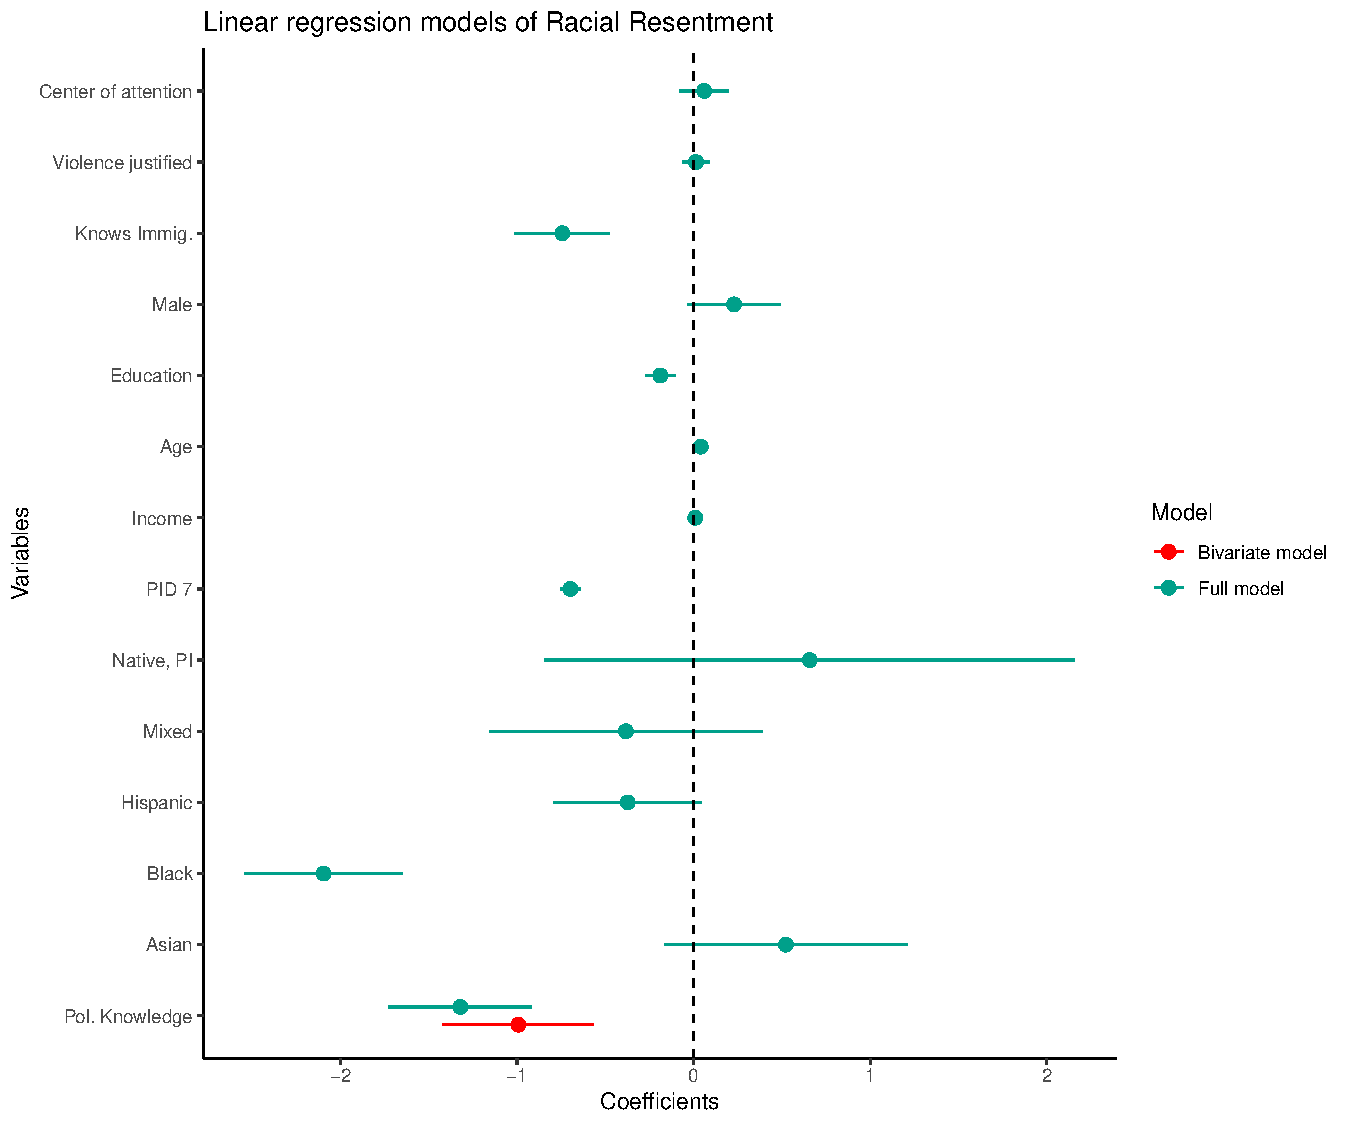
\includegraphics[width=0.7\linewidth]{../manuscript/figures/ols_coefficient_1.pdf}
\end{figure}
\end{frame}

\end{document}